\documentclass[paper=a4, fontsize=11pt]{scrartcl} % A4 paper and 11pt font size

\newcommand{\assignment}{2}
%\newcommand{\duedate}{January 25, 2023}
\usepackage[top=1in, bottom=1.5in, left=1in, right=1in]{geometry}
\usepackage{fancyhdr} % Required for custom headers
\usepackage{lastpage} % Required to determine the last page for the footer
\usepackage{extramarks} % Required for headers and footers
\usepackage[usenames,dvipsnames]{color} % Required for custom colors
\usepackage{graphicx} % Required to insert images
\usepackage{listings} % Required for insertion of code
\usepackage{courier} % Required for the courier font
\usepackage{amsmath}
\usepackage[super]{nth}
\usepackage{booktabs}
\usepackage[usenames,dvipsnames]{xcolor}
\usepackage{tcolorbox}
\usepackage{tabularx}
\usepackage{array}
\usepackage{colortbl}

%\usepackage[T1]{fontenc} % Use 8-bit encoding that has 256 glyphs
%\usepackage{fourier} % Use the Adobe Utopia font for the document - comment this line to return to the LaTeX default
\usepackage[english]{babel} % English language/hyphenation
\usepackage{amsmath,amsfonts,amsthm} % Math packages
\usepackage{graphicx}

\usepackage{hyperref}
\hypersetup{
  colorlinks   = true, %Colours links instead of ugly boxes
  urlcolor     = blue, %Colour for external hyperlinks
  linkcolor    = blue, %Colour of internal links
  citecolor   = red %Colour of citations
}

\usepackage{fancyhdr} % Custom headers and footers
\pagestyle{fancyplain} % Makes all pages in the document conform to the custom headers and footers
\fancyhead{} % No page header - if you want one, create it in the same way as the footers below
\fancyfoot[L]{} % Empty left footer
\fancyfoot[C]{} % Empty center footer
\fancyfoot[R]{\thepage} % Page numbering for right footer
\renewcommand{\headrulewidth}{0pt} % Remove header underlines
\renewcommand{\footrulewidth}{0pt} % Remove footer underlines
\setlength{\headheight}{13.6pt} % Customize the height of the header
\newcommand{\ts}{\textsuperscript}

\numberwithin{equation}{section} % Number equations within sections (i.e. 1.1, 1.2, 2.1, 2.2 instead of 1, 2, 3, 4)
\numberwithin{figure}{section} % Number figures within sections (i.e. 1.1, 1.2, 2.1, 2.2 instead of 1, 2, 3, 4)
\numberwithin{table}{section} % Number tables within sections (i.e. 1.1, 1.2, 2.1, 2.2 instead of 1, 2, 3, 4)

\setlength\parindent{0pt} % Removes all indentation from paragraphs - comment this line for an assignment with lots of text

% Default fixed font does not support bold face
\DeclareFixedFont{\ttb}{T1}{txtt}{bx}{n}{8} % for bold
\DeclareFixedFont{\ttm}{T1}{txtt}{m}{n}{8}  % for normal

%----------------------------------------------------------------------------------------
%	CODE BLOCKS
%----------------------------------------------------------------------------------------

\usepackage{adjustbox}
\usepackage{listings}
\usepackage{color}

\definecolor{dkgreen}{rgb}{0,0.6,0}
\definecolor{gray}{rgb}{0.5,0.5,0.5}
\definecolor{mauve}{rgb}{0.58,0,0.82}

\lstdefinelanguage{Dockerfile}
{
  morekeywords={FROM, RUN, CMD, LABEL, MAINTAINER, EXPOSE, ENV, ADD, COPY,
    ENTRYPOINT, VOLUME, USER, WORKDIR, ARG, ONBUILD, STOPSIGNAL, HEALTHCHECK,
    SHELL},
  morecomment=[l]{\#},
  morestring=[b]"
}

\lstset{
    columns=flexible,
    aboveskip=5mm,
    belowskip=5mm,
    keepspaces=true,
    showstringspaces=false,
    basicstyle=\ttfamily,
    commentstyle=\color{gray},
    keywordstyle=\color{purple},
    stringstyle=\color{green}
}



%----------------------------------------------------------------------------------------
%	TITLE SECTION
%----------------------------------------------------------------------------------------

\usepackage{eso-pic}
% \usepackage[demo]{graphicx}
\newcommand\AtPageUpperRight[1]{\AtPageUpperLeft{%
   \makebox[\paperwidth][r]{#1}}}

\newcommand{\horrule}[1]{\rule{\linewidth}{#1}} % Create horizontal rule command with 1 argument of height

\title{	
\normalfont \normalsize
\textsc{Northeastern University,  Khoury College of Computer Science} \\ [25pt] % Your university, school and/or department name(s)
\horrule{0.5pt} \\[0.4cm] % Thin top horizontal rule
\huge CS 6220  Data Mining \textemdash~Assignment \assignment \\ % The assignment title
\Large \textbf{Due: \duedate (100 points)} % The assignment title
\horrule{2pt} \\[0.5cm] % Thick bottom horizontal rule
}

% Original in the document
\AddToShipoutPictureBG*{%
  \AtPageUpperRight{\raisebox{-\height}{
\includegraphics[width=3cm]{images/logo}}}}

\author{
    \textbf{YOUR NAME} \\ 
    \textbf{YOUR GIT USERNAME} \\ 
    \textbf{YOUR E-MAIL}
}% INFORMATION

\date{} % Today's date or a custom date
% \author{
%     \textbf{YOUR NAME} \\ 
%     \textbf{YOUR GIT USERNAME} \\ 
%     \textbf{YOUR E-MAIL}
% }% INFORMATION

\begin{document}

\maketitle % Print the title

%%%%%%%%%%%%%%%%%%%%
\section{Getting Started}
%%%%%%%%%%%%%%%%%%%%
\subsection{Using Docker}
My Dockerfile is Figure 1.1 and I mainly set the python version and install related packages.
\begin{figure}[htbp]
    \centering
    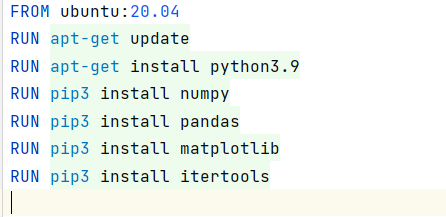
\includegraphics[width=400pt]{images/Q1_docker.png}
    \caption{Dockerfile}
    \label{fig:data-files}
    \end{figure}
Figure 1.2 shows the process of Dockerfile build. And Figure 1.3 show the already existed images list information. The first one is produced by me for this assignment.
\begin{figure}[htbp]
    \centering
    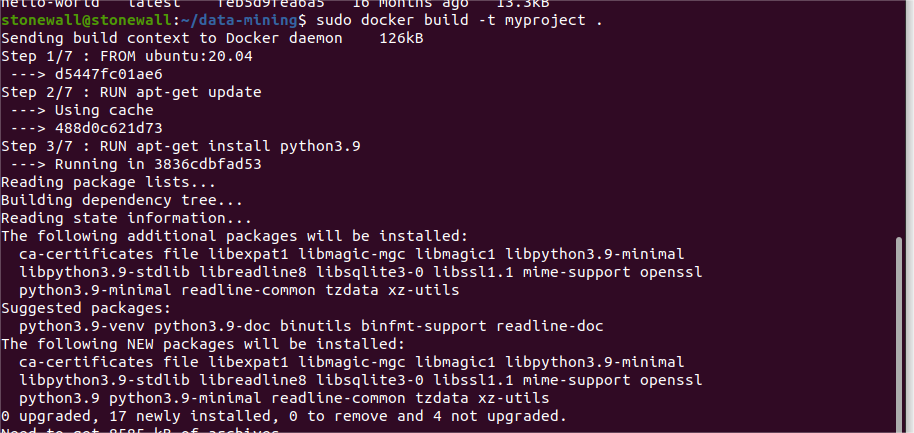
\includegraphics[width=400pt]{images/Q1_images_1_build.png}
    \caption{images build}
    \label{fig:data-files}
    \end{figure}
\begin{figure}[htbp]
    \centering
    
\includegraphics[width=400pt]{images/Q1_images_2_list.png}
    \caption{images list}
    \label{fig:data-files}
    \end{figure}
Figure 1.4 is container related information.
\begin{figure}[htbp]
    \centering
    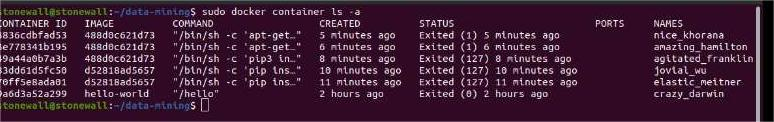
\includegraphics[width=400pt]{images/Q1_container.jpg}
    \caption{container}
    \label{fig:data-files}
    \end{figure}

%%%%%%%%%%%%%%%%%%%%
\section{Identifying All Sets}
%%%%%%%%%%%%%%%%%%%%
\subsection{}
 In this part, we use data structure set in python to select all different items. We can read all lines or line by line and split the line, strip the line. Then we can use union operation in set to filter all duplicated items. And we use the data set basket\_data.csv for testing and the corresponding result is 21.
    \begin{figure}[htbp]
    \centering
    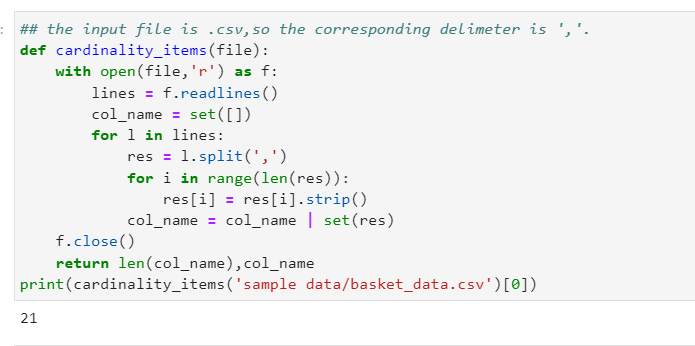
\includegraphics[width=400pt]{images/Q2_1.png}
    \caption{cardinality\_items}
    \label{fig:data-files}
    \end{figure}
    
 \subsection{}
 For each item, you have two choice select or not. And for N different items, the total combination number is $2^N$. When we ignore the null set and the final result is   
    $$2^N - 1$$
    
\subsection{}
\begin{figure}[htbp]
    \centering
    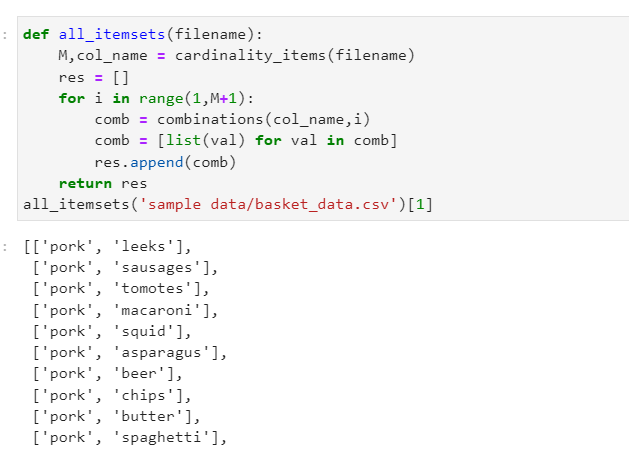
\includegraphics[width=400pt]{images/Q2_3.png}
    \caption{all\_itemsets}
    \label{fig:data-files}
    \end{figure}
Use the function cardinality\_items, we can obtain all different items. Then we can use function combinations in itertools to list all possible combinations.
    
  
\subsection{}
The main step is to count the total number of S repeated in D.
    \begin{figure}[htbp]
    \centering
    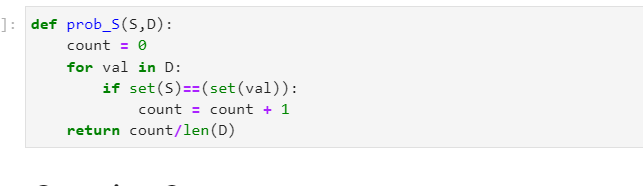
\includegraphics[width=400pt]{images/Q2_4.png}
    \caption{prob\_S}
    \label{fig:data-files}
    \end{figure}

    


%%%%%%%%%%%%%%%%%%%%
\section{The Netflix Challenge}
%%%%%%%%%%%%%%%%%%%%


%%%%%%%%%%%%%%%%%%%%
\subsection{Data Verification}
%%%%%%%%%%%%%%%%%%%%
From readme file, description of this data set are shown as below:
\begin{figure}[htbp]
    \centering
    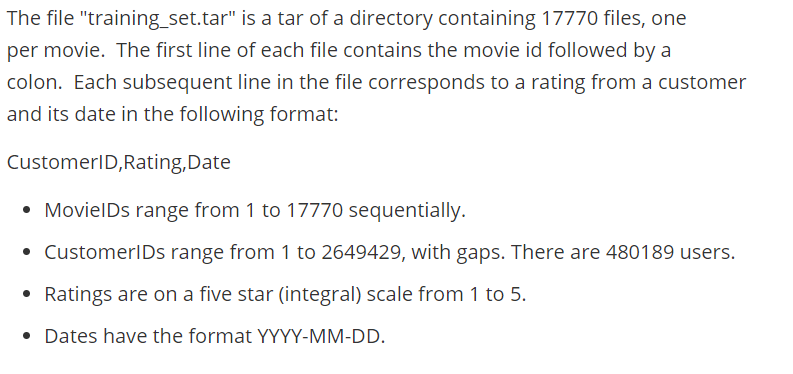
\includegraphics[width=400pt]{images/Q3_1_1_description.png}
    \caption{dataset description}
    \label{fig:data-files}
    \end{figure}
Therefore, the following code mainly verify these three aspects. Firstly, the four training dataset will be merged. From Figure 3.2, we can see that the column is right. Then verify the columns' range. Finally, from Figure 3.3, it can be found that verification passed. 
\begin{figure}[htbp]
    \centering
    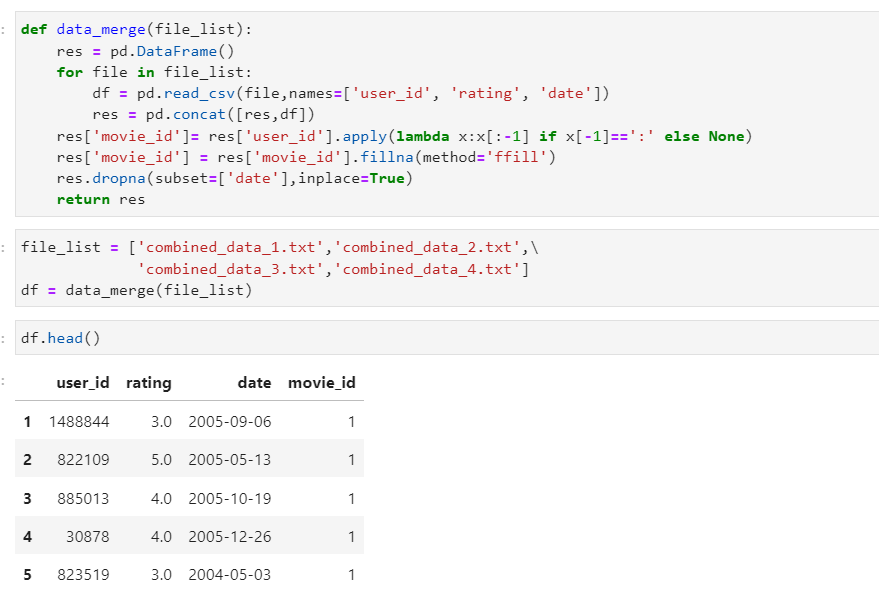
\includegraphics[width=400pt]{images/Q3_1_1_merge.png}
    \caption{dataset merge}
    \label{fig:data-files}
    \end{figure}
\begin{figure}[htbp]
    \centering
    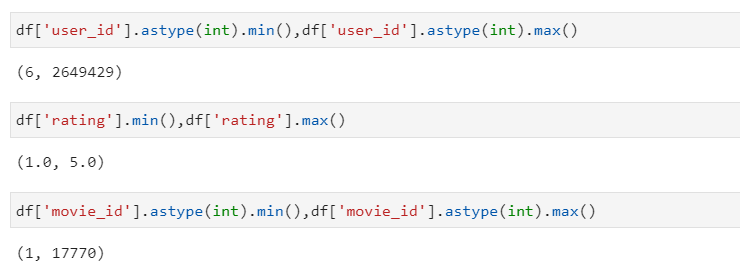
\includegraphics[width=400pt]{images/Q3_1_1_verify.png}
    \caption{range verification}
    \label{fig:data-files}
    \end{figure}




%%%%%%%%%%%%%%%%%%%%
\subsection{Data Analysis}
\label{sec:data-analysis}
%%%%%%%%%%%%%%%%%%%%

\subsubsection{}
There are total 100480507 records. From Figure 3.2, after dataset merge, examining its shape can count the number of records.
\begin{figure}[htbp]
    \centering
    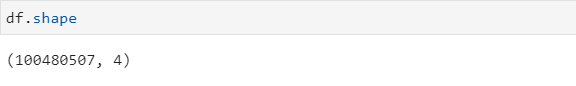
\includegraphics[width=400pt]{images/Q3_2_1.png}
    \caption{dataset shape examination}
    \label{fig:data-files}
    \end{figure}

\subsubsection{}
Towards this problem, all customers gave ratings in the same day will be computed their mean values. From the Figure 3.5, we can see there were great change around 1999. At that time, very excellent or bad movies occurred. Or there were some controversial movies. After that, the mean rating value tend to decrease slightly. But after 2004, the mean value became to increase.
\begin{figure}[htbp]
    \centering
    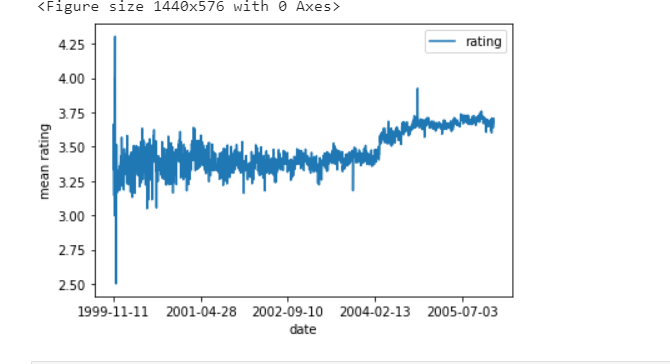
\includegraphics[width=400pt]{images/Q3_2_2.png}
    \caption{mean rating vs. date}
    \label{fig:data-files}
    \end{figure}

\subsubsection{}
Towards this problem, I will firstly give the concept of getting popular. In this experiment, I compute the mean rating stars of each year as corresponding value for that year. And then continue to compute their mean value as total mean value. Finally, using the total mean value subtract the first year rating
as the improvement value. If improvement is positive, we can evaluate the movie become popular. According to the definition, the percentage of the films have gotten more popular over time is 59.76\%.
\begin{figure}[htbp]
\centering
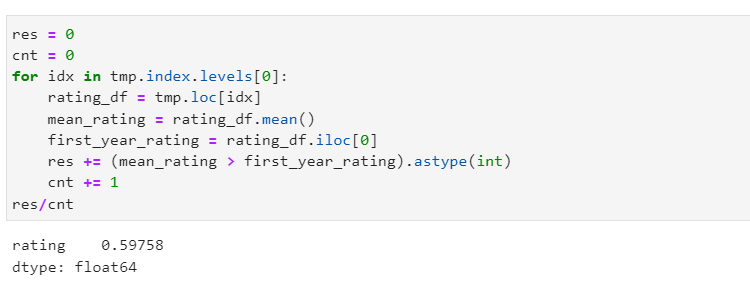
\includegraphics[width=400pt]{images/Q3_2_3.png}
\caption{percentage of the films become popular}
\label{fig:data-files}
\end{figure}

\subsubsection{}
For this problem, films re-released can be seen as file title occurring at least twice in movie\_title.csv. To simplify this step, we use duplicate function in pandas to count the result and 473 was obtained from Figure 3.7.
\begin{figure}[htbp]
\centering
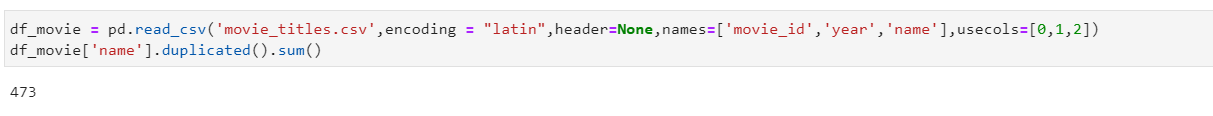
\includegraphics[width=400pt,height=60pt]{images/Q3_2_4.png}
\caption{number of films re-released}
\label{fig:data-files}
\end{figure}

\subsubsection{}
We may care about the type of different movies. In movie titles, we can extract its information about its type and we can explore the ratings over time and type. It may provide some useful information about which type of films are most popular nowadays.

\subsubsection{}
We may care about the interests of different customers. There are huge amount of records. If we can recommend someone a new movie according to similar interests shared by other people, it will provide better service. But there is still a challenge to deal with the computation cost.



\end{document}